% fig_method.tex -- Figure 1(a) of the IJCAI draft: overview of Upright kNN (TikZ, outlines only); test time on top, the ID-only training of the MLP below
\begin{tikzpicture}[font=\scriptsize, >={Stealth[length=1.5mm]},
  box/.style={draw, rounded corners=1.5pt, align=center, inner sep=2.2pt, minimum height=7.5mm},
  term/.style={box, line width=0.9pt},
  lab/.style={align=center, font=\tiny, inner sep=1pt}]
\node[inner sep=0] (x) {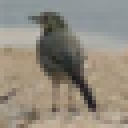
\includegraphics[width=0.95cm]{figs/ex_id.png}};
\node[below=0.4mm of x, inner sep=0] {image $\mathbf{x}$};
\node[box, right=7mm of x] (den) {frozen denoiser\\(one pass)};
\node[box, right=3mm of den] (feat) {last decoder block\\at 3 resolutions};
\coordinate (br) at ($(feat.east)+(2mm,0)$);
\node[box, anchor=west] (knn) at ($(br)+(15mm,8mm)$) {kNN: $R$-th similarity\\$c_R(\mathbf{x})$ to the bank};
\node[box, anchor=west, minimum width=25mm] (mlp) at ($(br)+(15mm,-8mm)$) {small MLP $q_\phi$};
\node[term, draw=navyc, right=2.5mm of knn] (t1) {$-d\log r_R(\mathbf{x})$\\{\tiny estimates $\log\bar p(\mathbf{x})$}};
\node[term, draw=redc, right=2.5mm of mlp] (t2) {$\log q_\phi(\Rot{0}\mid\mathbf{x})$\\{\tiny estimates $\log P(\mathrm{up}\mid\mathbf{x})$}};
\coordinate (mid) at ($(t1.east)!0.5!(t2.east)+(4mm,0)$);
\node[draw, circle, inner sep=0.8pt] (plus) at (mid) {$+$};
\node[right=1mm of plus, align=center] (s) {$s(\mathbf{x})$\\{\tiny ID score}};
\draw[->] (x) -- node[above, lab] {$+\sigma_1\veps$} (den);
\draw[->] (den) -- (feat);
\draw (feat.east) -- (br);
\draw[->] (br) |- node[pos=0.72, above, lab] {channel mean, std} (knn.west);
\draw[->] (br) |- node[pos=0.72, below, lab] {+ 2$\times$2 quadrants} (mlp.west);
\draw[->] (knn) -- (t1); \draw[->] (mlp) -- (t2);
\draw[->] (t1.east) -| (plus.north); \draw[->] (t2.east) -| (plus.south); \draw[->] (plus) -- (s);
\node[anchor=north east, align=left, inner sep=1pt] (trt) at ($(t2.south east)+(0,-5mm)$) {offline, ID images only ($\approx$10\,s): predict the angle $r$ of\\rotated bank images (\textbf{the noise is not rotated})};
\node[inner sep=0, left=2mm of trt] (r3) {\rotatebox{270}{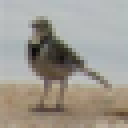
\includegraphics[width=0.42cm]{figs/ex_id_nn0.png}}};
\node[inner sep=0, left=0.7mm of r3] (r2) {\rotatebox{180}{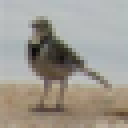
\includegraphics[width=0.42cm]{figs/ex_id_nn0.png}}};
\node[inner sep=0, left=0.7mm of r2] (r1) {\rotatebox{90}{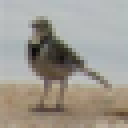
\includegraphics[width=0.42cm]{figs/ex_id_nn0.png}}};
\node[inner sep=0, left=0.7mm of r1] (r0) {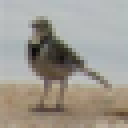
\includegraphics[width=0.42cm]{figs/ex_id_nn0.png}};
\node[draw, dashed, rounded corners=1.5pt, fit=(r0)(r3)(trt), inner sep=1.2mm] (tr) {};
\draw[->, dashed] (tr.north -| mlp.south) -- (mlp.south);
\end{tikzpicture}
